\chapter{Reinforcement Learning and Genetic Algorithms}
\label{chp:back_RLGA}

This chapter presents the theoretical background of reinforcement learning and genetic algorithms. A particular focus is given to the \ac{PPO} algorithm, which is the main algorithm used in the \ac{RL} framework of the codesign process implemented in this thesis. Finally, some novel approaches in the field of \ac{RL} are presented. This chapter are based on the work of \citet{sutton_reinforcement_1998,li_deep_2018,agarwal_deep_2022,holland_1992_ga}

\section{Fundamentals of Reinforcement Learning}

Reinforcement learning comes from a fusion of optimal control theory and the theory of machine learning and consists of guiding agents in dynamic environments to maximize cumulative rewards. Unlike supervised learning, \ac{RL} doesn't require labeled input/output pairs, and it focuses on striking a balance between exploring uncharted territory, and exploiting existing knowledge, from which come ideas of \textit{exploration} and \textit{exploitation}. Reinforcement learning's versatility extends to a wide range of disciplines like game theory, control theory, and swarm intelligence. Contrary to optimal control theory's emphasis on exact solutions, \ac{RL} addresses problems without a known mathematical model. Assessing an agent's performance against an optimally acting agent introduces the concept of regret, a measure from decision theory of the disparity between what the agent achieves and the best possible outcome, prompting a deeper understanding of the effectiveness and improvement potential within the learning process. For that, \ac{RL} excels in scenarios involving a trade-off between long-term and short-term rewards, requiring agents to consider the extended consequences of their actions. Overall, its adaptability makes it a powerful tool for complex problems that are difficult to model mathematically, such as multibody dynamics.

\begin{figure}
    \centering
    \caption{Reinforcement Learning Framework.}
    \label{fig:rlframework}
    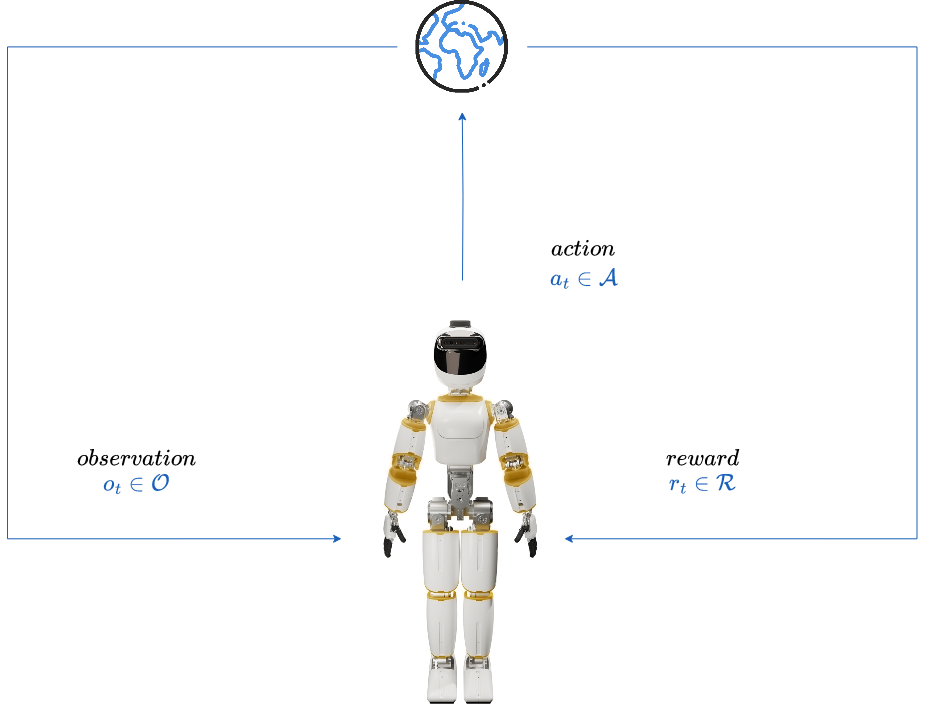
\includegraphics[width=.7\textwidth]{Images/rl_ergocub.png}
\end{figure}

\subsection{Key Mathematics}

\paragraph{Markov Decision Process} A \ac{MDP} is defined as a five-tuple $\mathcal{M} = (\mathcal{S}, \mathcal{A}, \mathcal{F}, r, \gamma)$ where:

\begin{itemize}
    \item $\mathcal{S}$ is the set of environment states $\mathbf{s} \in \mathcal{S}$, which may be either discrete or continuous
    \item $\mathcal{A}$ is the set of agent actions $\mathbf{a} \in \mathcal{A}$ which in a similar fashion may be continuous or discrete
    \item $\mathcal{F} (\mathbf{s}^\prime | \mathbf{s}, \mathbf{a}): \mathcal{S} \times \mathcal{A} \times \mathcal{S} \rightarrow \mathcal{S}$ is the state-transition function space that describes a conditional probability distribution $\mathcal{F}(\mathbf{s} _{t+1}|\mathbf{s}_t, \mathbf{a} _t)$ that describes the dynamics of the system
    \item $\mathcal{R} (\mathbf{s}^\prime, \mathbf{a}, \mathbf{s}): \mathcal{S} \times \mathcal{A} \times \mathcal{S} \rightarrow \mathbb{R}$ is the reward function
    \item $\gamma \in [0,1]$ is the discount factor that determines the weight of future rewards
\end{itemize}

If the environment is \textit{deterministic}, state transitions can be expressed with a state-transition function $\mathcal{F}: \mathcal{S} \times \mathcal{A} \times \mathcal{S} \rightarrow \mathcal{S}$, if the environment is \textit{stochastic}, state transitions can be expressed with the \textit{state-transition probability density function}, i.e. $\mathcal{F}: \mathcal{S} \times \mathcal{A} \times \mathcal{S} \rightarrow \mathbb{P}[\mathcal{S}]$.

As a reinforcement learning scenario has no prior knowledge regarding the data used for training, the state-transition map and the reward function are unknown.


\paragraph{Kullback-Leibler Divergence} The \ac{KL} divergence is a measure of how one probability distribution is different from a second, reference probability distribution. In other words, the \ac{KL} divergence measures the expected number of extra bits required to code samples from one distribution, given that we are using a code based on the reference distribution. The \ac{KL} divergence is defined as:

\begin{equation}
    \mathrm{KL}(P||Q) = \mathbb{E} _{x \sim P} \left[ \log \frac{P(x)}{Q(x)} \right] \qquad \in \left[0, \infty \right]
\end{equation}

where $P$ and $Q$ are two probability distributions. The \ac{KL} divergence is not symmetric, i.e. $\mathrm{KL}(P||Q) \neq \mathrm{KL}(Q||P)$. In the framework of reinforcement learning, it is commonly used to have a measure of how much the policy has changed from the previous iteration, in order to avoid too large policy updates, therefore what is actually seeked is the minimization of the \textit{reverse} \ac{KL} divergence $\mathrm{KL}(Q||P)$. In fact, in this mode-seeking behavior, the convergence will be achieved when the policy is close enough to the optimal policy, which is the one that maximizes the expected reward, i.e. when the \ac{KL} divergence is zero.

\subsection{Core Principles of Reinforcement Learning}

In general, a reinforcement learning process can be described as a \textit{partially observable Markov decision process}, in which the tuple describing the problem assumes the form $\mathcal{M} =  (\mathcal{S}, \mathcal{A}, \mathcal{O}, \mathcal{F}, r, \gamma)$, where the new variable $\mathcal{O}$ is defined as the observation space. For the purpose of this discussion and to simplify the notation, the training process will always be considered \textit{fully observable}, e.g. the observation space will be equal to the state space $\mathcal{O} = \mathcal{S}$.

At each time step $t$, the agent receives from the environment a state $\mathbf{s}_t \in \mathcal{S}$ and following a policy $\pi (\mathbf{a}_t | \mathbf{s}_t)$, outputs an action $\mathbf{a}_t \in \mathcal{A}$, as reported in \cref{fig:rlframework}. The environment will, via a transition function $\mathcal{F}$ output a reward $r_t \in \mathbb{R}$ and an observation $\mathbf{o} \in \mathcal{O}$, yielding an evolution of the state:

\begin{equation}
    \mathcal{F}(\mathbf{s} _{t+1}, r _{t+1} | \mathbf{s} _t, \mathbf{a} _t)
\end{equation}

in which $r_t \in \mathbb{R}$ is the reward at time $t$, or \textit{immediate reward}.
The reward function can be determined by the expected value of the immediate reward

\begin{equation}
    \label{eqn:reward_function}
    \mathcal{R}(\mathbf{s} _t, \mathbf{a} _t, \mathbf{s} _{t+1}) = \mathbb{E} \left[ r _t | \mathbf{s} _t, \mathbf{a} _t, \mathbf{s} _{t+1} \right] = \sum _t r _t \frac{\mathcal{F}(\mathbf{s} _{t+1}, r _{t+1} | \mathbf{s} _t, \mathbf{a} _t)}{\mathcal{F}(\mathbf{s} _{t+1} | \mathbf{s} _t, \mathbf{a} _t)}
\end{equation}

As the immediate reward depends on the state at time $t+1$, and therefore how action $\mathbf{a} _t$ affects the state at time $t$, we can define a \textit{return} $G _t$ as the total reward collected from time $t$ to the end of the episode:

\begin{equation}
    G _t = \sum ^{T - t} _{k = 0} r _{t+k+1}
\end{equation}

where $T$ is the final time step of the episode. As in continuous tasks the episode length is infinite, the return is usually defined as the discounted sum of rewards by introducing a discount factor $\gamma \in [0,1]$:

\begin{equation}
    \label{eqn:recursive_return}
    G _t = r_t + \gamma r _{t+1} + \gamma ^2 r _{t+2} + \dots = \sum ^{\infty} _{k = 0} \gamma ^k r _{t+k+1}
\end{equation}

From this definition, it is clear that when the discount factor is equal to $0$, the agent will only consider the immediate reward, while if it is equal to $1$, the agent will consider the total reward. In practice, the discount factor is usually set to a value close to $1$.

In \ac{DRL} the policy is described by a neural network, therefore it is modeled as a probability distribution parameterized by the set of the \ac{NN} weights and biases $\boldsymbol{\theta}$. In a standard \textit{Multi Layer Perceptron} policy, $\pi _{\boldsymbol{\theta}}(\mathbf{a} | \mathbf{s})$ is a multivariate Gaussian distribution with diagonal covariance matrix, i.e. $\pi _{\boldsymbol{\theta}}(\mathbf{a} | \mathbf{s}) = \mathcal{N}(\mu = \boldsymbol{\mu}(\mathbf{s}), \sigma = \boldsymbol{\sigma}(\mathbf{s}, \boldsymbol{\theta}))$, where $\mu$ and $\sigma$ are the mean and the standard deviation of the distribution, respectively. The policy is then defined as:

\begin{equation}
    \pi _{\boldsymbol{\theta}}(\mathbf{a} \mid \mathbf{s}) = \frac{1}{\sqrt{2 \pi \boldsymbol{\sigma} ^2}} \exp \left(- \frac{(\mathbf{a} - \boldsymbol{\mu}) ^2}{2 \boldsymbol{\sigma} ^2} \right)
\end{equation}

or, in terms of action space:

\begin{equation}
    a _t \sim \pi _{\boldsymbol{\theta}}(\cdot | s_t): \mathcal{S} \rightarrow \mathbb{P}(\mathcal{A})
\end{equation}

By defining the \textit{trajectory} generated by a policy $\pi$ a sequence of tuples state-action for a given episode of length $T$ as:

\begin{equation}
    h ^{\pi} = \left\{ (\mathbf{s} _0, \mathbf{a} _0), (\mathbf{s} _1, \mathbf{a} _1), \dots, (\mathbf{s} _{T-1}, \mathbf{a} _{T-1}), (\mathbf{s} _T) \right\}
\end{equation}

in which the initial state $\mathbf{s} _0$ gets sampled from the initial state distribution $p(\mathbf{s} _0)$.
In \textit{on-policy} method the policy is updated on the trajectory generated by the current policy, while in \textit{off-policy} methods the policy is updated on a trajectory generated by a different policy, therefore while on-policy methods like \ac{PPO} and \ac{TRPO} result in more stable training, off-policy methods like \ac{TD3} and \ac{SAC} are more sample efficient as they can sample from a \textit{replay buffer} of past trajectories.

Since the agent has no apriori knowledge on future rewards, it will try to learn a \textit{state-value function} $V(\mathbf{s})$ that estimates the expected return from a given state $\mathbf{s}$, where $\boldsymbol{\phi}$ is the set of parameters of the value function:

\begin{equation}
    V(\mathbf{s}) = \mathbb{E} _{h^{\pi}} \left[ G _t | \mathbf{s} _t = \mathbf{s} \right] = \mathbb{E} _{h^{\pi}} \left[ \sum ^{\infty} _{k = 0} \gamma ^k r _{t+k+1} | \mathbf{s} _t = \mathbf{s} \right]
\end{equation}

and will be then used to estimate the advantage of an action $\mathbf{a}$, e.g. a measure of how much an action can improve the expected return from a given state in the future.
If we define the \textit{action-value} function $Q(\mathbf{s}, \mathbf{a})$ as the expected return from a given state $\mathbf{s}$ and action $\mathbf{a}$:

\begin{equation}
    Q (\mathbf{s}, \mathbf{a}) = \mathbb{E} _{h^{\pi}} \left[ G _t | \mathbf{s} _t = \mathbf{s}, \mathbf{a} _t = \mathbf{a} \right] = \mathbb{E} _{h^{\pi}} \left[ \sum ^{\infty} _{k = 0} \gamma ^k r _{t+k+1} | \mathbf{s} _t = \mathbf{s}, \mathbf{a} _t = \mathbf{a} \right]
\end{equation}

then the advantage function can be defined as the difference between the action-value function and the state-value function, i.e. if an action $\mathbf{a}$ induces a state $\mathbf{s}$ producing a greater expected return, then the advantage will be negative, otherwise it will be positive:

\begin{equation}
    A (\mathbf{s}, \mathbf{a}) = Q (\mathbf{s}, \mathbf{a}) - V (\mathbf{s})
\end{equation}

Since the state-value function represents the expected return from a given state, it can be interpreted as a measure of how good a policy is, therefore the optimal policy $\pi ^*$ is the one that maximizes the state-value function. Similarly, the optimal action-value function $Q ^*$ is the one that maximizes the expected return from a given state-action pair:

\begin{equation}
    \pi ^* = \underset{\pi}{\arg\max} \ V (\mathbf{s}) \qquad Q ^* = \underset{\pi}{\arg\max} \ Q (\mathbf{s}, \mathbf{a})
\end{equation}

Recalling the recursive definition of the return presented in \cref{eqn:recursive_return} and the reward function definition in \cref{eqn:reward_function}, we can define the \textit{Bellman equation} \citep{bellman_dynamic_2003} for the state-value function as:

\begin{flalign}
    V (\mathbf{s}) & = \mathbb{E} _{h^{\pi}} \left[ G _t \mid \mathbf{s} \right] = \mathbb{E} _{h^{\pi}} \left[ r _t + \gamma G _{t+1} \mid \mathbf{s} \right]                                                                                                                         \\
                   & = \sum _{\mathbf{a}} \pi(\mathbf{a} \mid \mathbf{s})  \sum _{\mathbf{s} ^\prime \in \mathcal{S}} \mathcal{F}(\mathbf{s} ^\prime \mid \mathbf{s}) \left[\mathcal{R}(\mathbf{s} ^\prime, \mathbf{s}) + \gamma \mathbb{E} _{h^{\pi}} \right]  V (\mathbf{s} ^\prime)
\end{flalign}

and similarly for the action-value function:

\begin{flalign}
    Q (\mathbf{s}, \mathbf{a}) & = \mathbb{E} _{h^{\pi}} \left[ G_t \mid \mathbf{s}, \mathbf{a} \right]                                                                                                                                                                                                   \\
                               & = \mathbb{E} _{h^{\pi}} \left[ r _t + \gamma G_{t+1} \mid \mathbf{s}, \mathbf{a} \right]                                                                                                                                                                                 \\
                               & = \sum _{\mathbf{s} ^\prime \in \mathcal{S}} \mathcal{F}(\mathbf{s} ^\prime \mid \mathbf{s}, \mathbf{a}) \left[ \mathcal{R}(\mathbf{s} ^\prime, \mathbf{a}, \mathbf{s}) + \gamma \mathbb{E} _{h^{\pi}} \right] \left[ Q (\mathbf{s} ^\prime, \mathbf{a} ^\prime) \right]
\end{flalign}

\subsection{Policy Gradient Methods}

In continuous action spaces, as the optimal policy function $Q ^*(\mathbf{s}, \mathbf{a})$ is unknown, it is usually modeled as an optimized parametric function $\pi _{\theta}(\mathbf{a} | \mathbf{s})$ that outputs the probability of taking an action $\mathbf{a}$ in a state $\mathbf{s}$, where $\theta$ is the set of parameters of the policy. Therefrom, we can define a stochastic objective function $J(\theta)$ as the expected return of the policy $\pi _{\theta}$, being the return a random variable. Defining also the probability of a trajectory $h ^{\pi}$ as the probability of the initial state $s _0$ times the probability of the action $a _0$ times the probability of the next state $s _1$ and so on, e.g.

\begin{equation}
    \mathbb{P}(h ^{\pi}) = \mathbb{P}(s _0) \mathbb{P}(a _0 | s _0) \mathbb{P}(s _1 | s _0, a _0) \dots = \mathbb{P}(s _0) \prod ^{\infty} _{t = 0} \pi _{\theta} (a _t | s _t) \mathbb{P}(s _{t+1} | s _t, a _t)
\end{equation}

we can define the objective function as:

\begin{equation}
    J(\theta) = \mathbb{E} _{\pi _{\theta}} \left[ G _t \right] = \mathbb{E} _{\pi _{\theta}} \left[ \sum ^{\infty} _{k = 0} \gamma ^k r _{t+k+1} \right]
\end{equation}

from which we can derive the policy update rule once defined the policy gradient:

\begin{equation}
    \theta _{t+1} = \theta _t + \alpha \nabla _{\theta} J(\pi)
\end{equation}

where $\alpha \in \mathbb{R} ^+$ is the learning rate. The policy gradient is then defined as:

\begin{equation}
    \nabla _{\theta} J(\pi) = \nabla _{\theta} \int _{h ^{\pi}} \mathbb{P}(h ^{\pi})G(h ^{\pi})dh ^{\pi} = \dots = \mathbb{E} _{h^{\pi}} \left[ \sum ^{\infty} _{k = 0} \gamma ^k \nabla _{\theta} \log \pi _{\theta} (a _t | s _t) G _t \right]
\end{equation}

\subsubsection{Proximal Policy Optimization}

Amongst policy gradient methods, the \textit{Proximal Policy Optimization} (\ac{PPO}) is by far one of the most used and effective algorithms. It is a family of first-order methods that use a \textit{surrogate objective} in order to ensure a \textit{trust region} on the policy update.
Moreover, being an \textit{actor-critic} method, it uses two neural networks, one for learning the policy and one for learning the value function, acting as a feedback  loop for the policy network.

The version of \ac{PPO} adopted in this work uses a clipped surrogate objective and introduces a penalization term on the \ac{KL} divergence between the new and the old policy, ensuring small policy updates that would otherwise lead to unstable training, once defined:

\begin{equation}
    \mathfrak{R} _t (\boldsymbol{\theta}) = \frac{\pi_{\boldsymbol{\theta}} (\mathbf{a}_t \mid \mathbf{s}_t)}{\pi _{\boldsymbol{\theta}_{\text{old}}} (\mathbf{a}_t \mid \mathbf{s}_t)}
\end{equation}

resulting in the following formulation:

\begin{equation}
    \mathcal{L} (\boldsymbol{\theta}) = \hat{\mathbb{E}} \left[\min \left\{ \mathfrak{R}_t(\boldsymbol{\theta}) \hat{A}_t, \text{clip}\left(\mathfrak{R}_t(\boldsymbol{\theta}) , 1- \varepsilon, 1+\varepsilon \right)  \right\} - \beta \mathrm{KL} [\pi_{\boldsymbol{\theta}_{\text{old}}} (\cdot \mid \mathbf{s}_t), \pi_{\boldsymbol{\theta}} (\cdot \mid \mathbf{s}_t) ] \right]
\end{equation}

in which the $\text{clip}$ operator bounds the first argument in the interval $[1-\varepsilon, 1+\varepsilon]$, $\varepsilon$ is the clipping coefficient, $\hat{\mathbb{E}}$ is the empirical expectation, $\hat{A}_t$ is the advantage estimate at time $t$ and $\beta$ is the penalty coefficient for the KL divergence.


% The most common optimizer for \ac{NN} parameters is the first-order gradient-based optimization of stochastic objective function update ADAM \citep{kingma_adam_2017}, reported in \cref{alg:adam}, which
% updates exponential moving averages of the two gradients, where $\beta_1$ and $\beta_2$ control the decay rates of the moving averages, which are then estimates of the first and second raw moment, corresponding respectively to the mean and uncentered variance.

% \begin{algorithm}[H]
%     \caption{ADAM}
%     \label{alg:adam}
%     \begin{algorithmic}[1]
%         \Require learning rate $\gamma$, exponential decay rates for the moment estimates $\beta_1, \beta_2$, initial parameter vector $\theta_0$, stochastic objective $f(\theta)$, weight decay $\lambda$
%         \Require $m_0 \leftarrow 0, v_0 \leftarrow 0$
%         \For{$t = 1$ \textbf{to} convergence}
%         \If{$\lambda \neq 0$}
%         \State $g_t \leftarrow g_t + \lambda\theta_{t-1}$
%         \EndIf
%         \State $g_t \leftarrow \nabla _{\theta} f_t (\theta_{t-1}$)
%         \State $m_t \leftarrow \beta_1 m_{t-1} + (1-\beta_1)g_t$
%         \State $\hat{m_t} \leftarrow \beta_1 m_{t-1} + (1-\beta_1)g_t$
%         \State $\hat{v_t} \leftarrow v_t / (1-\eta_2 ^\top)$
%         \State $\theta_t \leftarrow \theta_t - \gamma \hat{m_t} / (\sqrt{\hat{v}} + \varepsilon)$
%         \EndFor
%         \Return $\theta_t$
%     \end{algorithmic}
% \end{algorithm}

\begin{algorithm}[H]
    \caption{Clipped Proximal Policy Optimization.}
    \label{alg:ppo}
    \begin{algorithmic}[1]
        \Require Initial policy parameters $\theta _0$, initial value
        \For{$k = 0,1,2, \dots$}
        \State Collect set of trajectories $\mathcal{D} _k = \tau _i$ by running policy $\pi _k = \pi(\theta _k)$in the environment
        \State Compute rewards-to-go $\hat{R} _t$
        \State Compute advantage estimates $\hat{A} _t$
        (using any method of advantage estimation) based on the current value function $V _{\phi _k}$
        \State Update policy by maximizing the PPO-Clip objective:
        $$
            \theta _{k + 1} = \underset{\theta}{\arg\max} = \frac{1}{|\mathcal{D} _k|T} \sum _{r \in \mathcal{D} _k} \sum _{t = 0} ^{T} \min \left( \frac{\pi _{\theta} (a _t | s _t)}{\pi _{\theta_k} (a _t | s _t)} A ^{\pi _{\theta_k}} (s _t, a _t), g(\varepsilon, A ^{\pi _{\theta_k}}(s _t, a _t)) \right)
        $$
        typically via Stochastic gradient ascent. Where:
        $$
            \hat{g} = \hat{\mathbb{E}} _t \left[\nabla _{\theta}\log\pi _{\theta}(a _t | s _t) \hat{A} _t\right]
        $$
        \State Fit value function by regression on mean-squared error
        $$
            \phi _{k + 1} = \underset{\phi}{\arg\min} = \frac{1}{|\mathcal{D} _k|T} \sum _{r \in \mathcal{D} _k} \sum _{t = 0} ^{T} \left(V _{\phi}(s _t) - \hat{R} _t \right)^2
        $$
        typically via some gradient descent algorithm.
        \EndFor
    \end{algorithmic}
\end{algorithm}


\paragraph{State Dependent Exploration} Likelihood ratio methods such as \ac{PPO} suffer from high variance due to random exploration at every time step of each training episode, used to introduce some \textit{domain randomization} and produce more stable policies. Yet, an alternative is represented by \ac{SDE} \citep{daelemans_state-dependent_2008, raffin_smooth_2021} which adds a \textit{state-dependent offset} to actions at each timestep that will the same value in the state state within an episode, but it will vary between episodes.

Given a pseudo-random function $\hat{\varepsilon}(\mathbf{x}, \hat{\theta})$ where $\hat{\theta} \sim \mathcal{N}(0, \hat{\sigma} _j ^2)$, the action is computed as:

\begin{equation}
    \mathbf{a} = f(\mathbf{x}, \boldsymbol{\theta}) + \hat{\varepsilon}(\mathbf{x}, \hat{\theta})
\end{equation}

% Should I explain how this gets updated?

Therefore the usual approximation with finite differences of the gradient cannot be computed. Thus, the expectation is approximated e.g. by \textit{Monte-Carlo sampling}, which yields \citep{williams_simple_1992} the episodic gradient estimation:

\begin{equation}
    \nabla _{\boldsymbol{\theta}} J(\pi) = \frac{1}{N} \sum _{h^{\pi}} \sum ^{T-1} _{t = 0} \nabla _{\boldsymbol{\theta}} \log \pi(a _t | h _t ^{\pi}) R(h ^{\pi})
\end{equation}

% Yet, as perturbed action leads to a stochastic policy which in general is not differentiable due to the high variance in the gradient estimation, therefore it is usually approximated with the finite difference method:

% \begin{equation}
%     \label{eqn:finitediff}
%     \frac{\partial J(\boldsymbol{\theta})}{\partial \theta _i} \approx \frac{J(\boldsymbol{\theta} + \delta \boldsymbol{\theta}) - J(\boldsymbol{\theta})}{\delta \theta _i}
% \end{equation}

\paragraph{Generalized Advantage Estimate}
By defining the \textit{generalized advantage estimator} (\ac{GAE}) or \textit{temporal difference estimate} as in \cite{schulman_high-dimensional_2018}:

\begin{equation}
    \hat{A}(s,a) = r _0 + \gamma \hat{V}(s _1) - \hat{V}(s _0)
\end{equation}

this can be modified to be less biased by taking $n$ steps for each update, this will also scale the magnitude of the value estimate adding a time-sensitivity:

\begin{equation}
    \hat{A} ^{(n)} (s,a) = r _0 + \gamma r _1 + \dots + \gamma ^{n-1} r _{n-1} + \gamma ^n \hat{V}(s _n) - \hat{V}(s _0)
\end{equation}

yet computing its expected value, it can be shown that this has an increased variance.

A potentially good solution might be to take the exponential average as input to the \textit{extended advantage estimator} $\hat{A} ^{(i)}(s, a) $, where $i$ is a number between $1$ and $n$ that cuts the summation of the \textit{temporal difference advantage} to the $i$-th term. Letting $\delta _t$ be the \textit{temporal difference advantage estimate} for the timestep $t$:

\begin{align}
    \hat{A} _t ^{\text{GAE} (\gamma, \lambda)} & := (1 - \lambda)(\hat{A} _t ^{(1)} + \lambda \hat{A} _t ^{(2)} + \lambda ^2 \hat{A} _t ^{(3)} + \dots) \\
                                               & = \dots \nonumber                                                                                      \\
                                               & = \sum ^{ \infty } _{l = 0} (\gamma \lambda) ^\top \delta ^V _{t+l} \nonumber
\end{align}

where $\lambda$ is the exponential weight discount. If this is set to $0$, then we have exactly the \ac{TD} advantage estimate (high bias, low variance) and if we set it to $1$, this is equivalent to choosing $i=n$ for the extended advantage estimate (low bias, high variance).

\section{Fundamentals of Evolutionary Algorithms}

Evolutionary algorithm or \textit{Genetic Algorithm}s (\ac{GA}) is a family of powerful optimization algorithms that are inspired by the natural selection
process and genetics, in which some individuals are selected to reproduce and pass their characteristics to the next generation, according to some evaluation metrics. Rooted in evolutionary computation, these algorithms emulate the process of natural selection to evolve solutions for complex problems. Introduced by \citet{holland_1992_ga}, genetic algorithms are particularly effective when dealing with complex, non-linear, and multi-dimensional search spaces, finding near-optimal solutions in diverse domains. Their ability to explore diverse solution spaces, without the need for differentiability, and to adapt to changing environments makes them valuable tools in the optimization field. \citep{katoch_review_2021}

The core idea behind genetic algorithms involves representing potential solutions to a problem as individuals in a population. Through successive generations, these individuals undergo genetic operations mimicking the mechanisms of biological evolution. As the algorithm progresses, the fittest individuals, those with higher adaptability or better solutions, are more likely to survive and contribute to the next generation.

A generic evolutionary algorithm starts with an initial population of individuals, chosen randomly or according to some heuristic, then the first two individuals are randomly picked from the population and combined to generate a new individual in a process called \textit{crossover}. As evolutionary algorithm are prone to get stuck in local minima, filling the population with sub-optimal individuals and therefore preventing the algorithm from finding the global optimum, a certain percentage of the population is  mutated with a certain probability and added to the population if fit enough. The process is repeated until a stopping criterion is met, e.g. a maximum number of generations is reached or the fitness of the population is above a certain threshold. An overview of the evolutionary process can be found in \cref{fig:genetic_algo}.

\begin{figure}
    \centering
    \caption{Evolutionary Algorithm Flowchart.}
    \label{fig:genetic_algo}
    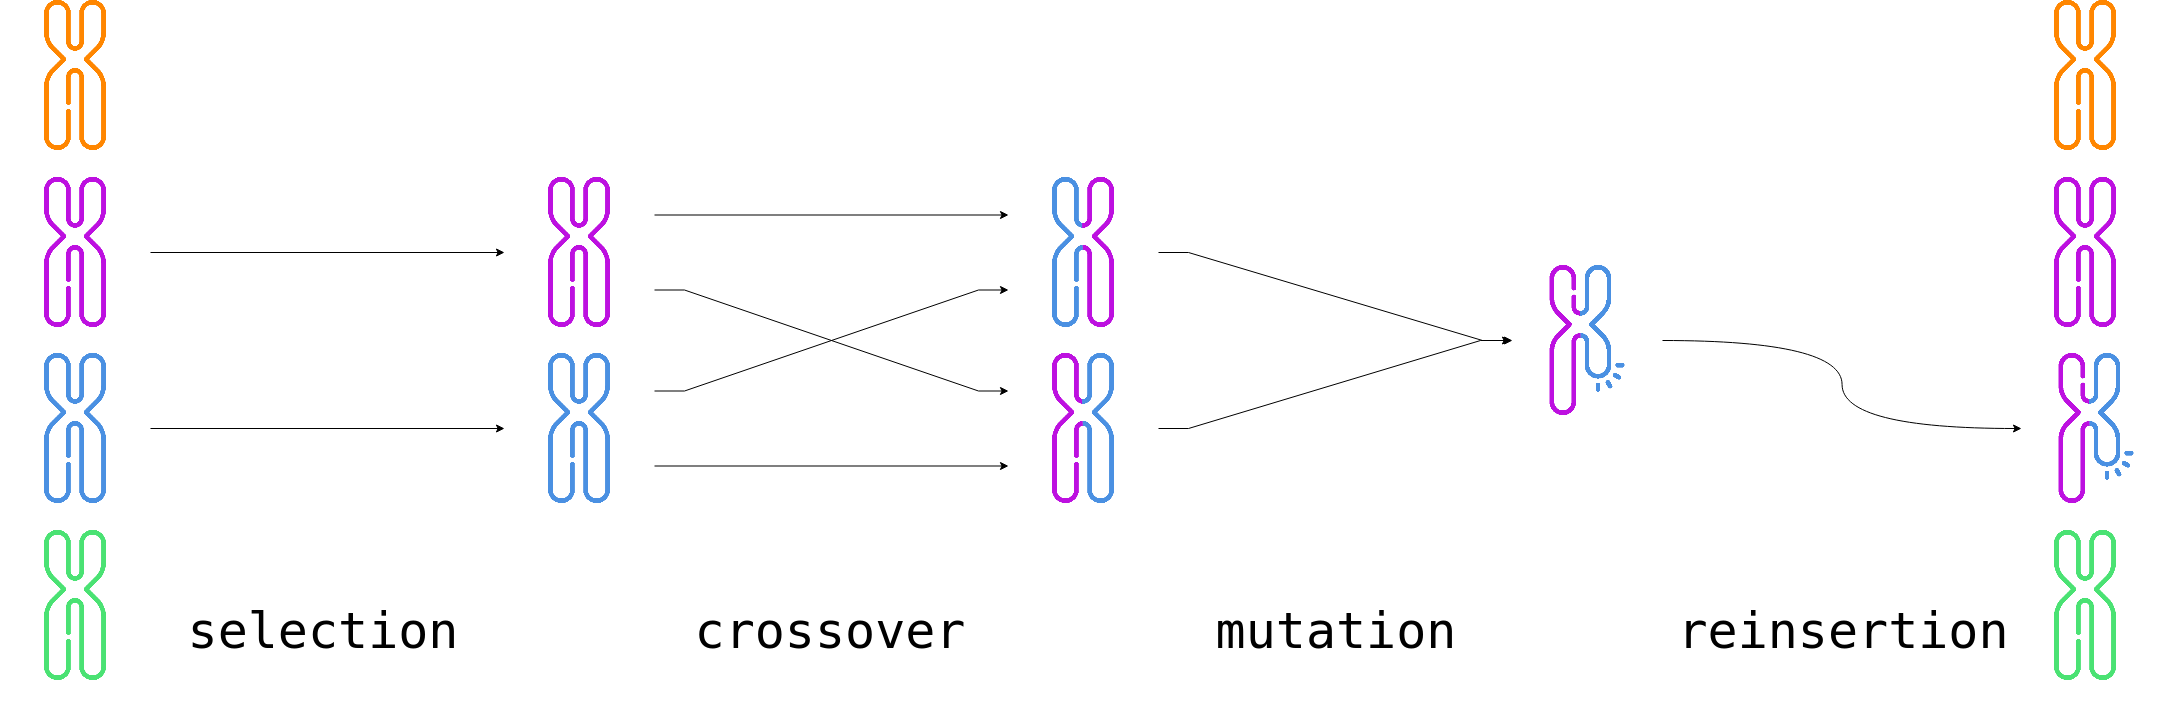
\includegraphics[width=.9\textwidth]{Images/genetic_algo.png}
\end{figure}

\subsection{Genetic Operators}

\paragraph{Tournament Selection}

Tournament selection is a strategy to select individuals for reproduction in which a subset of individuals is selected from the population and the fittest individual is chosen from the subset.

\paragraph{Mutation}

Mutation is a genetic operator used to introduce new genetic information into the population. In practice, the individual characteristic is modified by applying a random perturbation to its genetic information. The mutation happens with a certain probability, called \textit{mutation rate}, which needs to be tuned as a too high mutation rate can lead to a loss of genetic information, preventing the algorithm to reach convergence, while a too low mutation rate can lead to a stagnation of the algorithm.

\paragraph{Elitism}

Elitism is a selection strategy in which the fittest individuals are preserved from one generation to the next. It is used to ensure that the fittest individuals are not lost during the evolution process and to speed up the convergence of the algorithm.

\paragraph{Crossover}

Crossover is a genetic operator used to combine the genetic information of two individuals to generate a new individual. In the context of evolutionary algorithms, crossover is used to generate new individuals from the population. The crossover operator is inspired by the natural reproduction process, in which the genetic information of two individuals is combined to generate a new individual. A generic \textit{k-point crossover} operator takes two individuals and a number $k$ as input and returns two new individuals. The two individuals are divided into $k+1$ segments, and the segments are then swapped between the two individuals.